%\section{Sở GD Đồng Nai --Lần 1 NH: 2025--2026}
\vspace{-0.5cm}
\Opensolutionfile{ans}[ans/ans-26-2-DongNai-SoGD-L1]
\caulc

\begin{ex}%[1H8N7-3]
	Cho hình chóp $S.ABCD$ có đáy là hình vuông cạnh bằng $a$, $SA \perp (ABCD)$, $SA=a\sqrt{3}$. Thể tích khối chóp $S.ABCD$ bằng
	\choice
	{$a^{3}\sqrt{3}$}
	{$\dfrac{a^{3}}{3}$}
	{\True $\dfrac{a^{3}\sqrt{3}}{3}$}
	{$a^{3}$}
	\loigiai{
		\immini{
			Đáy $ABCD$ là hình vuông cạnh $a$ nên diện tích đáy là $S_{ABCD} = a^2$.\\
			Vì $SA \perp (ABCD)$ nên $SA$ là chiều cao của khối chóp.\\
			$h = SA = a\sqrt{3}$.\\
			Thể tích khối chóp $S.ABCD$ là:
			$$V = \dfrac{1}{3} S_{ABCD} \cdot SA = \dfrac{1}{3} \cdot a^2 \cdot a\sqrt{3} = \dfrac{a^3\sqrt{3}}{3}.$$
		}{
			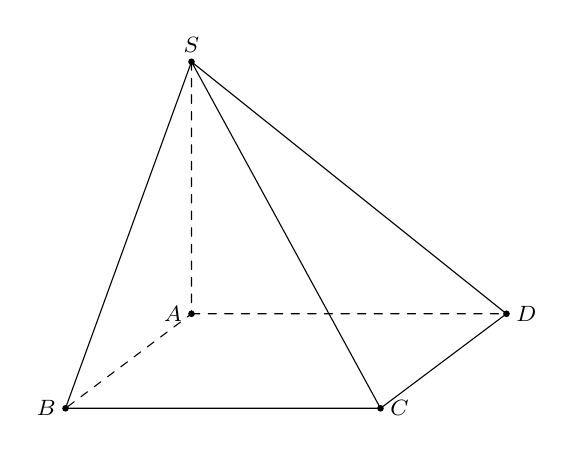
\begin{tikzpicture}[>=stealth,line join=round,line cap=round,font=\footnotesize,scale=0.8]
				\coordinate (A) at (0,0);
				\coordinate (B) at (-2,-1.5);
				\coordinate (C) at (3,-1.5);
				\coordinate (D) at (5,0);
				\coordinate (S) at (0,4);
				\draw (S)--(B)--(C)--(D)--(S)--(C);
				\draw[dashed] (S)--(A)--(B) (A)--(D);
				\draw[dashed, black] (S)--(A); % Highlight chiều cao như hình gốc
				\fill (S) circle (1.5pt) node[above] {$S$};
				\fill (A) circle (1.5pt) node[left] {$A$};
				\fill (B) circle (1.5pt) node[left] {$B$};
				\fill (C) circle (1.5pt) node[right] {$C$};
				\fill (D) circle (1.5pt) node[right] {$D$};
			\end{tikzpicture}
		}
	}
\end{ex}

\begin{ex}%[2D4H3-1]
	\immini{
		Gọi $S$ là diện tích hình phẳng giới hạn bởi các đường $y=f(x)$, trục hoành và hai đường thẳng $x=-3$, $x=2$, như hình vẽ bên. Đặt $a=\displaystyle\int\limits_{-3}^{1}f(x)\mathrm{\,d}x$, $b=\displaystyle\int\limits_{1}^{2}f(x)\mathrm{\,d}x$. Mệnh đề nào sau đây là đúng?
	}{
		\begin{tikzpicture}[>=stealth,x=1cm,y=1cm,scale=0.8]
			\draw[->] (-4.5,0) -- (3.5,0) node[below] {$x$};
			\draw[->] (0,-3.5) -- (0,2.5) node[left] {$y$};
			\node[above left] at (0,0) {$0$};
			\draw[fill=black] (-3,0) circle (1.5pt) node[above] {$-3$};
			\draw[fill=black] (1,0) circle (1.5pt) node[above left] {$1$};
			\draw[fill=black] (2,0) circle (1.5pt) node[below right] {$2$};
			
		\draw[thick] plot[smooth] coordinates {
			(-3.5,-3) (-3.3,-2.6) (-3,-2) (-2.7,-1.5) (-2.3,-1) (-1.9,-0.7) (-1.5,-0.5) (-1,-0.35) (-0.5,-0.25) (0,-0.2) (0.5,-0.12) (1,0) (1.3,0.3) (1.6,0.7) (1.8,1.1) (2,1.5) (2.2,1.9) (2.35,2.2) (2.5,2.5)};
			\fill[pattern=north east lines] (-3,0) -- plot[smooth] coordinates {(-3,-2) (-2.7,-1.5) (-2.3,-1) (-1.9,-0.7) (-1.5,-0.5) (-1,-0.35) (-0.5,-0.25) (0,-0.2) (0.5,-0.12) (1,0) } -- cycle;
			\fill[pattern=north east lines] (1,0) -- plot[smooth] coordinates {(1,0) (1.3,0.3) (1.6,0.7) (1.8,1.1) (2,1.5)} -- (2,0) -- cycle;
			
			\draw[dashed, opacity=0.5] (-3,0) -- (-3,-2);
			\draw[dashed, opacity=0.5] (2,0) -- (2,1.5);
			
		\end{tikzpicture}
	}
	\choice
	{$S=-a-b$}
	{$S=a+b$}
	{\True $S=b-a$}
	{$S=a-b$}
	\loigiai{
		Dựa vào đồ thị, ta thấy trên đoạn $[-3;1]$, đồ thị hàm số $y=f(x)$ nằm phía dưới trục hoành nên $f(x) \le 0$. Suy ra $|f(x)| = -f(x)$.\\
		Trên đoạn $[1;2]$, đồ thị hàm số $y=f(x)$ nằm phía trên trục hoành nên $f(x) \ge 0$. Suy ra $|f(x)| = f(x)$.\\
		Diện tích hình phẳng $S$ được tính bởi công thức:
			\allowdisplaybreaks
			\begin{align*}
				S &= \displaystyle\int\limits_{-3}^{2}|f(x)|\mathrm{\,d}x = \displaystyle\int\limits_{-3}^{1}|f(x)|\mathrm{\,d}x + \displaystyle\int\limits_{1}^{2}|f(x)|\mathrm{\,d}x \\
				&= \displaystyle\int\limits_{-3}^{1}\left[-f(x)\right]\mathrm{\,d}x + \displaystyle\int\limits_{1}^{2}f(x)\mathrm{\,d}x \\
				&= -\displaystyle\int\limits_{-3}^{1}f(x)\mathrm{\,d}x + \displaystyle\int\limits_{1}^{2}f(x)\mathrm{\,d}x \\
				&= -a + b = b - a
			\end{align*}
	}
\end{ex}

\begin{ex}%[2H5N1-4]
	Trong không gian $Oxyz$, mặt phẳng $(P)\colon x+5y-2z-2=0$ song song với mặt phẳng nào dưới đây?
	\choice
	{\True $2x+10y-4z+1=0$}
	{$x-5y+2z+2=0$}
	{$x+5y-2z-2=0$}
	{$-x-5y-2z+2=0$}
	\loigiai{
			Xét mặt phẳng ở đáp án A: $(Q)\colon 2x+10y-4z+1=0$.\\
			Xét tỉ số các hệ số tương ứng của $(Q)$ và $(P)$, ta có:
			$$ \dfrac{2}{1} = \dfrac{10}{5} = \dfrac{-4}{-2} \neq \dfrac{1}{-2} $$
			Vậy mặt phẳng $(Q)$ song song với mặt phẳng $(P)$.\\
	}
\end{ex}

\begin{ex}%[1D2H2-3]
	Cho cấp số cộng $(u_n)$ thỏa mãn $\heva{&u_{4}=10\\ &u_{4}+u_{6}=26}$. Công sai của $(u_n)$ là
	\choice
	{$d=-3$}
	{\True $d=3$}
	{$d=6$}
	{$d=5$}
	\loigiai{
		Chuyển đổi hệ giả thiết về ẩn $u_1$ và $d$:
		\begin{align*}
			\heva{&u_{4}=10\\ &u_{4}+u_{6}=26} &\Leftrightarrow \heva{&u_1+3d=10\\ &(u_1+3d)+(u_1+5d)=26} \\
			& \Leftrightarrow \heva{&u_1+3d=10\\ &2u_1+8d=26} \\
			& \Leftrightarrow \heva{&u_1=1\\ &d=3.}
		\end{align*}
		Vậy công sai của cấp số cộng là $d=3$.
	}
\end{ex}
\begin{ex}%[1D6H4-2]
	Tổng bình phương các nghiệm của phương trình $\log_{2}(x^{2}-5x+7)=0$ bằng
	\choice
	{$6$}
	{$7$}
	{\True $13$}
	{$5$}
	\loigiai{
		 Biến đổi phương trình đã cho, ta được:
			\begin{align*}
				\log_2(x^2-5x+7) = 0 &\Leftrightarrow x^2 - 5x + 7 = 2^0 \\
				&\Leftrightarrow x^2 - 5x + 7 = 1 \\
				&\Leftrightarrow x^2 - 5x + 6 = 0. \\
				&\Leftrightarrow \left[\begin{aligned} &x = 2 \\ &x = 3. \end{aligned}\right.
			\end{align*}
		Vậy phương trình có hai nghiệm là $x=2$ và $x=3$.
		Tổng bình phương các nghiệm của phương trình là $2^2 + 3^2 = 4 + 9 = 13$.\\
	}
\end{ex}

\begin{ex}%[2D4N1-1]
	Hàm số $F(x)$ được gọi là một nguyên hàm của hàm số $f(x)$ trên khoảng $K$ nếu
	\choice
	{$f^{\prime}(x)=-F(x)$, $\forall x\in K$}
	{$f^{\prime}(x)=F(x)$, $\forall x\in K$}
	{\True $F^{\prime}(x)=f(x)$, $\forall x\in K$}
	{$F^{\prime}(x)=-f(x)$, $\forall x\in K$}
	\loigiai{
		Dựa vào định nghĩa nguyên hàm, hàm số $F(x)$ là nguyên hàm của hàm số $f(x)$ trên khoảng $K$ khi và chỉ khi:
			$$ F^{\prime}(x)=f(x), \forall x\in K $$
		Đối chiếu với các phương án, ta thấy phương án đúng là $F^{\prime}(x)=f(x)$, $\forall x\in K$.
	}
\end{ex}

\begin{ex}%[2H2N1-2]
	\immini{
		Cho hình hộp $ABCD.A'B'C'D'$ (tham khảo hình bên). Gọi $M$, $N$ lần lượt là trung điểm của các cạnh $BC$ và $CD$. Vectơ nào sau đây bằng $2\vec{MN}$
		\choice
		{$\vec{A'C'}$}
		{$\vec{AD}$}
		{\True $\vec{B'D'}$}
		{$\vec{BC}$}
	}{
		\begin{tikzpicture}[scale=1, font=\footnotesize, line join=round, line cap=round]
			\coordinate (D) at (0,0);
			\coordinate (C) at (3.5,0);
			\coordinate (A) at (-1.5,1.2);
			\coordinate (B) at (2,1.2);
			\coordinate (D') at (-0.5,2.5);
			\coordinate (C') at (3,2.5);
			\coordinate (A') at (-2,3.7);
			\coordinate (B') at (1.5,3.7);
			\coordinate (M) at ($(B)!0.5!(C)$);
			\coordinate (N) at ($(C)!0.5!(D)$);
			
			\draw (A) -- (D) -- (C) -- (C') -- (B') -- (A') -- cycle;
			\draw (A') -- (D') -- (C');
			\draw (D) -- (D');
			\draw[dashed] (A) -- (B) -- (C);
			\draw[dashed] (B) -- (B');
			\draw[dashed, ->, >=stealth, black] (M) -- (N);
			
			\fill (A) circle (1.5pt) node[left] {$A$};
			\fill (B) circle (1.5pt) node[right] {$B$};
			\fill (C) circle (1.5pt) node[right] {$C$};
			\fill (D) circle (1.5pt) node[below left] {$D$};
			\fill (A') circle (1.5pt) node[left] {$A'$};
			\fill (B') circle (1.5pt) node[above] {$B'$};
			\fill (C') circle (1.5pt) node[right] {$C'$};
			\fill (D') circle (1.5pt) node[above right] {$D'$};
			\fill (M) circle (1.5pt) node[right] {$M$};
			\fill (N) circle (1.5pt) node[below] {$N$};
		\end{tikzpicture}
	}
	\loigiai{
		Xét tam giác $BCD$, ta có $M, N$ lần lượt là trung điểm của $BC, CD$.\\
		Suy ra $MN$ là đường trung bình của tam giác $BCD$.\\
		Do đó $\vec{MN} = \dfrac{1}{2}\vec{BD} \Leftrightarrow 2\vec{MN} = \vec{BD}$.\\
		Mặt khác, vì $ABCD.A'B'C'D'$ là hình hộp nên $BB'D'D$ là hình bình hành, dẫn đến $\vec{BD} = \vec{B'D'}$.\\
		Vậy $2\vec{MN} = \vec{B'D'}$.\\
	}
\end{ex}



\begin{ex}%[Dự án EX chương trình 2025]%[Nhóm Toán & \TeX]%[1H4H3-2]
	\immini{
		Cho hình chóp $S.ABCD$ có đáy $ABCD$ là hình chữ nhật (tham khảo hình bên). Gọi $M$, $N$ theo thứ tự là trọng tâm tam giác $SAB$ và tam giác $SCD$. Khi đó $MN$ song song với mặt phẳng nào sau đây?
	}{
		\begin{tikzpicture}[scale=1, font=\footnotesize, line join=round, line cap=round, >=stealth]
			\coordinate (A) at (0,0);
			\coordinate (D) at (5,0);
			\coordinate (B) at (-2,-2);
			\coordinate (C) at (3,-2);
			\coordinate (S) at (1,3);
			\coordinate (E) at ($(A)!0.5!(B)$);
			\coordinate (F) at ($(C)!0.5!(D)$);
			\coordinate (M) at ($(S)!2/3!(E)$);
			\coordinate (N) at ($(S)!2/3!(F)$);
			
			\draw (S)--(B)--(C)--(D)--(S)--(C);
			\draw (S)--(F);
			\draw[dashed] (S)--(A)--(B) (A)--(D);
			\draw[dashed] (S)--(E) (M)--(N);
			
			\draw [fill=black] (S) circle (1pt) node[above] {$S$};
			\draw [fill=black] (A) circle (1pt) node[below right] {$A$};
			\draw [fill=black] (B) circle (1pt) node[left] {$B$};
			\draw [fill=black] (C) circle (1pt) node[right] {$C$};
			\draw [fill=black] (D) circle (1pt) node[right] {$D$};
			\draw [fill=black] (M) circle (1pt) node[above left] {$M$};
			\draw [fill=black] (N) circle (1pt) node[right] {$N$};
		\end{tikzpicture}
	}
	\choice
	{$(SBD)$}
	{$(SAB)$}
	{$(SAC)$}
	{\True $(ABCD)$}
	\loigiai{
		\begin{center}
			\begin{tikzpicture}[scale=1, font=\footnotesize, line join=round, line cap=round, >=stealth]
				% Định vị các đỉnh của hình chóp
				\coordinate (A) at (0,0);
				\coordinate (D) at (5,0);
				\coordinate (B) at (-2,-2);
				\coordinate (C) at (3,-2);
				\coordinate (S) at (1,3);
				
				% Xác định trung điểm và trọng tâm
				\coordinate (E) at ($(A)!0.5!(B)$);
				\coordinate (F) at ($(C)!0.5!(D)$);
				\coordinate (M) at ($(S)!2/3!(E)$);
				\coordinate (N) at ($(S)!2/3!(F)$);
				
				% Vẽ các nét thấy (liền)
				\draw (S)--(B)--(C)--(D)--(S)--(C);
				\draw (S)--(F); % SF nhìn thấy vì nằm trên mặt phẳng (SCD)
				
				% Vẽ các nét khuất (đứt)
				\draw[dashed] (S)--(A)--(B) (A)--(D);
				\draw[dashed] (M)--(N) (E)--(F); % MN và EF đều là nét đứt
				\draw[dashed] (S)--(E); % SE nhìn thấy vì nằm trên mặt phẳng (SAB)
				
				% Vẽ và hiển thị tên các điểm đặt cuối để không bị đường thẳng đè lên
				\draw [fill=black] (S) circle (1pt) node[above] {$S$};
				\draw [fill=black] (A) circle (1pt) node[below right] {$A$};
				\draw [fill=black] (B) circle (1pt) node[left] {$B$};
				\draw [fill=black] (C) circle (1pt) node[below right] {$C$};
				\draw [fill=black] (D) circle (1pt) node[right] {$D$};
				\draw [fill=black] (E) circle (1pt) node[below right] {$E$};
				\draw [fill=black] (F) circle (1pt) node[below right] {$F$};
				\draw [fill=black] (M) circle (1pt) node[above left] {$M$};
				\draw [fill=black] (N) circle (1pt) node[right] {$N$};
			\end{tikzpicture}
		\end{center}
		Gọi $E$, $F$ lần lượt là trung điểm của $AB$, $CD$.\\
		Vì $M$, $N$ lần lượt là trọng tâm của các tam giác $SAB$ và $SCD$ nên $M \in SE$, $N \in SF$ và ta có tỉ số
		$$ \dfrac{SM}{SE} = \dfrac{2}{3}; \quad \dfrac{SN}{SF} = \dfrac{2}{3} \Rightarrow \dfrac{SM}{SE} = \dfrac{SN}{SF}. $$
		Xét tam giác $SEF$, có $\dfrac{SM}{SE} = \dfrac{SN}{SF}$ nên theo định lý Thales đảo ta có $MN \parallel EF$.\\
		Mặt khác, $E$, $F$ là trung điểm của các cạnh đối diện của hình chữ nhật $ABCD$ nên $EF \subset (ABCD)$.\\
		Vì $MN \parallel EF$, $EF \subset (ABCD)$ và $MN \not\subset (ABCD)$ nên $MN \parallel (ABCD)$.\\
	}
\end{ex}



\begin{ex}%[2H5H3-3]
	Trong không gian $Oxyz$, mặt cầu có tâm $I(2;1;-4)$ và tiếp xúc với mặt phẳng $(\alpha)\colon x-2y+2z-7=0$ có phương trình là
	\choice
	{\True $(x-2)^{2}+(y-1)^{2}+(z+4)^{2}=25$}
	{$(x+2)^{2}+(y+1)^{2}+(z-4)^{2}=25$}
	{$(x+2)^{2}+(y-1)^{2}+(z+4)^{2}=25$}
	{$(x-2)^{2}+(y-1)^{2}+(z-4)^{2}=25$}
	\loigiai{
		Vì mặt cầu tiếp xúc với mặt phẳng $(\alpha)$ nên bán kính mặt cầu chính là khoảng cách từ tâm $I$ đến mặt phẳng $(\alpha)$.\\
		Bán kính mặt cầu là: $R =\mathrm{d}(I, (\alpha)) = \dfrac{|2 - 2 \cdot 1 + 2 \cdot (-4) - 7|}{\sqrt{1^2 + (-2)^2 + 2^2}} = \dfrac{|-15|}{\sqrt{9}} = \dfrac{15}{3} = 5$.\\
		Phương trình mặt cầu có tâm $I(2;1;-4)$ và bán kính $R=5$ là: $(x-2)^2 + (y-1)^2 + (z+4)^2 = 25$.
	}
\end{ex}
\begin{ex}%[1D5H1-3]
	Thống kê cân nặng của học sinh lớp 12A ở một trường THPT ta có bảng số liệu sau:
	\begin{center}
		\begin{tabular}{|l|c|c|c|c|c|c|}
			\hline
			Cân nặng & $[40{,}5; 45{,}5)$ & $[45{,}5; 50{,}5)$ & $[50{,}5; 55{,}5)$ & $[55{,}5; 60{,}5)$ & $[60{,}5; 65{,}5)$ & $[65{,}5; 70{,}5)$ \\ \hline
			Số học sinh & $10$ & $7$ & $16$ & $4$ & $2$ & $3$ \\ \hline
		\end{tabular}
	\end{center}
	Tìm số trung bình của bảng số liệu.
	\choice
	{$51{,}80$}
	{\True $51{,}81$}
	{$51{,}809$}
	{$52$}
	\loigiai{
		Chọn giá trị đại diện cho từng nhóm số liệu, ta có bảng phân bố tần số ghép nhóm sau:
			\begin{center}
				\begin{tabular}{|l|c|c|c|c|c|c|}
					\hline
					Cân nặng & $[40{,}5; 45{,}5)$ & $[45{,}5; 50{,}5)$ & $[50{,}5; 55{,}5)$ & $[55{,}5; 60{,}5)$ & $[60{,}5; 65{,}5)$ & $[65{,}5; 70{,}5)$ \\ \hline
					Giá trị đại diện & $43$ & $48$ & $53$ & $58$ & $63$ & $68$ \\ \hline
					Số học sinh & $10$ & $7$ & $16$ & $4$ & $2$ & $3$ \\ \hline
				\end{tabular}
			\end{center}
		Cỡ mẫu $N = 10 + 7 + 16 + 4 + 2 + 3 = 42$.\\
		Số trung bình của bảng số liệu ghép nhóm là:
			$$
			\bar{x} = \dfrac{10 \cdot 43 + 7 \cdot 48 + 16 \cdot 53 + 4 \cdot 58 + 2 \cdot 63 + 3 \cdot 68}{42}
			= \dfrac{2176}{42} \approx 51{,}81.
			$$
	}
\end{ex}

\begin{ex}%[1D1N5-3]
	Nghiệm của phương trình $\cos x=1$ là
	\choice
	{$x=\dfrac{k\pi}{2}$ $(k\in\mathbb{Z})$}
	{$x=k\pi$ $(k\in\mathbb{Z})$}
	{$x=\dfrac{\pi}{2}+k2\pi$ $(k\in\mathbb{Z})$}
	{\True $x=k2\pi$ $(k\in\mathbb{Z})$}
	\loigiai{
		Áp dụng công thức nghiệm của phương trình lượng giác cơ bản đối với trường hợp đặc biệt, ta có
			$$\cos x = 1 \Leftrightarrow x = k2\pi \quad (k \in \mathbb{Z}).$$
		Vậy nghiệm của phương trình là $x = k2\pi$ $(k \in \mathbb{Z})$.
	}
\end{ex}

\begin{ex}%[2D1H5-1]
	\immini{
		Đường cong trong hình vẽ bên là đồ thị của hàm số nào sau đây?
		\choice
		{\True $y=\dfrac{x^{2}+2x+2}{x+1}$}
		{$y=\dfrac{x^{2}+3x}{x-2}$}
		{$y=\dfrac{x^{2}-2x-3}{x-2}$}
		{$y=\dfrac{x^{2}-2x}{x+1}$}
	}{
		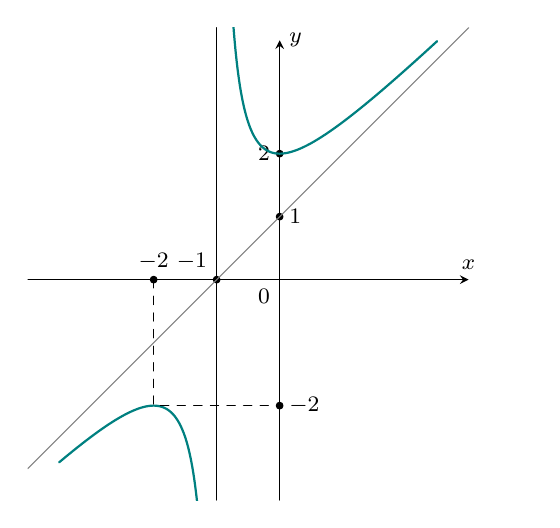
\begin{tikzpicture}[>=stealth,line join=round,line cap=round,font=\footnotesize,scale=0.8]
			\clip (-4,-3.5) rectangle (4,4);
			\draw[->] (-4,0) -- (3,0) node[above] {$x$};
			\draw[->] (0,-3.5) -- (0,3.8) node[right] {$y$};
			\node[below left] at (0,0) {$0$};
			\draw[fill=black] (-2,0) circle (1.5pt) node[above] {$-2$};
			\draw[fill=black] (-1,0) circle (1.5pt) node[above left] {$-1$};
			\draw[fill=black] (0,2) circle (1.5pt) node[left] {$2$};
			\draw[fill=black] (0,1) circle (1.5pt) node[right] {$1$};
			\draw[fill=black] (0,-2) circle (1.5pt) node[right] {$-2$};
			\draw (-1,-3.5) -- (-1,4);
			\draw[gray, thin] (-4,-3) -- (3,4);
			\draw[thick, teal] plot[smooth, domain=-3.5:-1.2, samples=100] (\x, {(\x*\x+2*\x+2)/(\x+1)});
			\draw[thick, teal] plot[smooth, domain=-0.8:2.5, samples=100] (\x, {(\x*\x+2*\x+2)/(\x+1)});
			\draw[dashed] (-2,0) -- (-2,-2) -- (0,-2);
		\end{tikzpicture}
	}
	\loigiai{
		Dựa vào đồ thị, ta thấy đường thẳng $x = -1$ là tiệm cận đứng của đồ thị hàm số.\\
		Từ đó, ta loại phương án B và C vì hàm số ở hai phương án này có tiệm cận đứng là $x=2$.\\
		Tiếp tục quan sát đồ thị, ta thấy đồ thị đi qua điểm $(0; 2)$.\\
		Thử tọa độ điểm $(0; 2)$ vào hai hàm số còn lại ở phương án A và D.\\
		Với $y=\dfrac{x^{2}+2x+2}{x+1}$, thay $x=0$ ta được $y = \dfrac{0+0+2}{0+1} = 2$ (thỏa mãn).\\
		Với $y=\dfrac{x^{2}-2x}{x+1}$, thay $x=0$ ta được $y = \dfrac{0-0}{0+1} = 0 \neq 2$ (loại).\\
		Vậy đường cong trong hình là đồ thị của hàm số $y=\dfrac{x^{2}+2x+2}{x+1}$.\\
	}
\end{ex}
\Closesolutionfile{ans}

\cauds
\Opensolutionfile{ans}[ans/ans-26-2-DongNai-SoGD-L1-DS]

\begin{ex}[] %[] %[]%[2H2H2-6]
	Một ống dẫn nước $OAB$ được cố định vào một bức tường đồng thời được đặt trong hệ toạ độ $Oxyz$ và có các kích thước như hình vẽ.
	\begin{center}
		\begin{tikzpicture}[font=\footnotesize, x={(-0.6cm,-0.4cm)}, y={(1cm,0cm)}, z={(0cm,1cm)}, scale=0.8]
			% Draw wall
			\fill[gray!20] (-1,0,-2) -- (6,0,-2) -- (6,0,7) -- (-1,0,7) -- cycle;
			\draw[gray] (-1,0,-2) -- (6,0,-2) -- (6,0,7) -- (-1,0,7) -- cycle;
			
			% Axes
			\draw[->, >=stealth, blue] (0,0,0) -- (7,0,0) node[below] {$x$};
			\draw[->, >=stealth, blue] (0,0,0) -- (0,12,0) node[right] {$y$};
			\draw[->, >=stealth, blue] (0,0,0) -- (0,0,8) node[above] {$z$};
			
			% Points
			\coordinate (O) at (0,0,0);
			\coordinate (A) at (0,10,0);
			\coordinate (B) at (3,10,-5.196); % -3*sqrt(3)
			\coordinate (C) at (4,0,5);
			\coordinate (B_proj) at (3,10,0);
			
			% Dimensions
			\draw[<->, >=stealth, dashed, gray] (4,0,0) -- (C) node[midway, left] {$5$ dm};
			\draw[<->, >=stealth, dashed, gray] (0,0,0) -- (4,0,0) node at (2,0,-0.2) [below] {$4$ dm};
			\draw[<->, >=stealth, dashed, gray] (O) -- (0,10,0) node[midway, above] {$10$ dm};
			\draw[<->, >=stealth, dashed, gray] (A) -- (3,10,0) node at (2.5,10,0) [right]  {$3$ dm (hình chiếu)};
			\draw[<->, >=stealth, dashed, gray] (3,10,0) -- (B) node at (3,11,-2) [right] {$6$ dm (chiều dài thật)};
			
			% Pipes
			\draw[line width=4pt, gray!70] (O) -- (A);
			\draw[line width=4pt, gray!70] (A) -- (B);
			\fill[gray!90] (A) circle (2pt);
			\fill[gray!90] (O) circle (3pt);
			
			% Points and wire
			\draw[dashed] (A) -- (3,10,0);
			\draw[dashed] (B) -- (3,10,0);
			
			\draw[thick, gray!80!black] (C) -- (B);
			
			% Angle
			\draw[dashed] (A) -- (4,10,0);
			\draw (1.7,10,0) arc (0:-115:1) node at (0.1,9.2,0) [below] {$60^\circ$};
			
			% Labels
			\node[below] at (0,0,-0.2) {$O$};
			\node[above] at (A) {$A$};
			\node[below] at (B) {$B$};
			\node[left] at (C) {$C$};
			\fill (C) circle (1.5pt);
			\fill (B) circle (1.5pt);
		\end{tikzpicture}
	\end{center}
	\begin{itemize}
		\item Đoạn ống $OA$ nằm trên tia $Oy$ (vuông góc với tường), có chiều dài $OA=10$ dm.
		\item Đoạn ống $AB$ nối tiếp với $OA$, có chiều dài $AB=6$ dm. Ống $AB$ vuông góc với $OA$ và hướng xuống dưới, tạo với mặt phẳng nằm ngang $(Oxy)$ một góc $60^\circ$.
		\item Đầu $B$ của ống được giữ cố định bởi một thanh sắt nối với điểm $C$ trên tường. Biết điểm $C(4;0;5)$. (Đơn vị trên các trục là dm).
	\end{itemize}
	\choiceTF[t]
	{\True Hình chiếu vuông góc của điểm $B$ lên mặt phẳng $(Oyz)$ là điểm $H(0;10;-3\sqrt{3})$}
	{\True Tọa độ của điểm $A(0;10;0)$}
	{Cao độ của điểm $B$ là $-3$}
	{Độ dài thanh sắt $BC$ là $14,1$ dm}
	\loigiai{
		\begin{itemize}
			\item Vì đoạn ống $OA$ nằm trên tia dương $Oy$ và $OA = 10$ dm nên tọa độ điểm $A$ là $(0; 10; 0)$.
			\item Ống $AB$ vuông góc với $OA$ (chính là trục $Oy$) nên $AB$ nằm trong mặt phẳng đi qua $A$ và song song với mặt phẳng $(Oxz)$ (mặt phẳng $y = 10$). Do đó tung độ của $B$ là $y_B = y_A = 10$.
			\item Ống $AB$ tạo với mặt ngang $(Oxy)$ một góc $60^\circ$ và hướng xuống dưới. Gọi $A'$ là điểm sao cho $AA'$ song song và cùng chiều với trục $Ox$, khi đó góc $\widehat{BAA'} = 60^\circ$.
			\item Hoành độ của $B$ được tính bằng độ dài hình chiếu của đoạn $AB$ lên phương song song với trục $Ox$:
			$$x_B = x_A + AB \cdot \cos 60^\circ = 0 + 6 \cdot \dfrac{1}{2} = 3.$$
			\item Cao độ của $B$ được tính bằng độ dài hình chiếu của $AB$ lên phương thẳng đứng (mang dấu âm vì hướng xuống dưới trục $Oz$):
			$$z_B = z_A - AB \cdot \sin 60^\circ = 0 - 6 \cdot \dfrac{\sqrt{3}}{2} = -3\sqrt{3}.$$
			\item Vậy tọa độ điểm $B$ là $(3; 10; -3\sqrt{3})$.
		\end{itemize}
		\begin{itemchoice}
			\itemch Hình chiếu vuông góc của điểm $B$ lên mặt phẳng $(Oyz)$ là điểm $H(0;10;-3\sqrt{3})$.
			\begin{itemize}
				\item Hình chiếu vuông góc của điểm $B(3; 10; -3\sqrt{3})$ lên mặt phẳng $(Oyz)$ có tọa độ là $(0; y_B; z_B)$.
				\item Vậy hình chiếu là điểm $H(0; 10; -3\sqrt{3})$.
			\end{itemize}
			
			\itemch Tọa độ của điểm $A(0;10;0)$.
			\begin{itemize}
				\item Dựa vào bước lập luận ban đầu, $A$ nằm trên tia $Oy$ và cách gốc tọa độ $10$ dm nên $A(0; 10; 0)$.
			\end{itemize}
			
			\itemch Cao độ của điểm $B$ là $-3$.
			\begin{itemize}
				\item Tọa độ điểm $B$ vừa tìm được là $(3; 10; -3\sqrt{3})$.
				\item Vậy cao độ của điểm $B$ là $-3\sqrt{3}$, khác với $-3$.
			\end{itemize}
			
			\itemch Độ dài thanh sắt $BC$ là $14{,}1$ dm.
			\begin{itemize}
				\item Đề bài cho tọa độ điểm $C(4; 0; 5)$. Ta áp dụng công thức tính khoảng cách hai điểm $B(3; 10; -3\sqrt{3})$ và $C$:
				$$BC = \sqrt{(3-4)^2 + (10-0)^2 + (-3\sqrt{3}-5)^2}\approx 14{,}316 \text{ (dm).} $$
			\end{itemize}
		\end{itemchoice}
	}
\end{ex}

\begin{ex}%[Sưu tầm]%[Dự án EX]%[2D4V2-6]
	Có hai chất điểm $A$, $B$ đang chuyển động thì xảy ra va chạm. Biết rằng sau khi va chạm hai chất điểm di chuyển về hai hướng ngược nhau, chất điểm $A$ di chuyển tiếp với tốc độ $v_1(t)=6-3t$ (m/s), chất điểm $B$ di chuyển với tốc độ $v_2(t)=12-4t$ (m/s) trước khi cả hai dừng lại, $t$ là thời gian tính bằng giây, thời điểm ban đầu $t=0$ là lúc xảy ra va chạm.
	\begin{center}
		\begin{tikzpicture}[scale=0.8, font=\footnotesize, line join=round, line cap=round, >=stealth]
			% Phần 1: Trước va chạm
			\node[right] at (-6.5,2.5) {\textbf{PHẦN 1} (Trước va chạm)};
			\draw (-6.5,1.2) -- (6.5,1.2);
			\shade[ball color=blue] (-5.5,1.6) circle (0.4) node[white] {\textbf{A}};
			\draw[->,blue,thick] (-5.1,1.6) -- (-2,1.6) node[midway,above] {$\overrightarrow{v}_1'$};
			\shade[ball color=orange] (5.5,1.6) circle (0.4) node[white] {\textbf{B}};
			\draw[->,orange,thick] (5.1,1.6) -- (2,1.6) node[midway,above] {$\overrightarrow{v}_2'$};
			\draw[dashed] (0,-2.5) -- (0,3);
			
			% Va chạm - Làm nhỏ ngôi sao bằng cách dùng văn bản nhỏ hơn và giảm inner sep
			\node[
			star,
			star points=10,
			star point ratio=2,
			fill=red,
			draw=orange,
			inner sep=1pt,
			scale=0.5
			] at (0,0.5)
			{\color{white}\scriptsize\shortstack{\textbf{VA CHẠM} \\ \textbf{(COLLISION)}}};
			
			% Phần 2: Sau va chạm
			\node[right] at (-6.5,-0.5) {\textbf{PHẦN 2} (Sau va chạm)};
			\draw (-6.5,-1.8) -- (6.5,-1.8);
			\shade[ball color=blue] (-1.5,-1.4) circle (0.4) node[white] {\textbf{A}};
			\draw[->,blue,thick] (-1.9,-1.4) -- (-4.5,-1.4) node[midway,above] {$\overrightarrow{v}_1$};
			\shade[ball color=orange] (1.5,-1.4) circle (0.4) node[white] {\textbf{B}};
			\draw[->,orange,thick] (1.9,-1.4) -- (4.5,-1.4) node[midway,above] {$\overrightarrow{v}_2$};
		\end{tikzpicture}
	\end{center}
	\choiceTFt
	{Quãng đường chất điểm $A$ di chuyển được kể từ khi va chạm đến khi dừng lại là $18$ m}
	{\True Sau va chạm chất điểm $A$ dừng lại sau $2$ s}
	{\True Quãng đường chất điểm $A$ di chuyển sau khi va chạm đến khi dừng hẳn được biểu diễn bởi hàm số $s_1(t)=6t-\dfrac{3}{2}t^2$ (m)}
	{Khoảng cách hai chất điểm sau khi đã dừng hẳn là $23$ m}
	\loigiai{
		\begin{itemchoice}
			\itemch Thời gian chất điểm $A$ di chuyển từ lúc va chạm đến khi dừng lại thỏa mãn
			$v_1(t)=0 \Leftrightarrow 6-3t=0 \Leftrightarrow t=2$. \\
			Quãng đường chất điểm $A$ di chuyển được từ lúc va chạm đến lúc dừng hẳn là
			$$s_1 = \displaystyle\int\limits_0^2 v_1(t) \mathrm{\,d}t = \displaystyle\int\limits_0^2 (6-3t) \mathrm{\,d}t = \left(6t-\dfrac{3}{2}t^2\right)\bigg|_0^2 = 6 \text{ m}.$$
			Do đó, phát biểu sai.
			\itemch Theo tính toán ở ý trên, thời gian chất điểm $A$ di chuyển từ lúc va chạm đến khi dừng lại là $t=2$ s. \\
			Do đó, phát biểu đúng.
			\itemch Hàm số biểu diễn quãng đường di chuyển của chất điểm $A$ kể từ lúc va chạm là một nguyên hàm của hàm vận tốc $v_1(t)$.
			Ta có $s_1(t) = \displaystyle\int v_1(t) \mathrm{\,d}t = \displaystyle\int (6-3t) \mathrm{\,d}t = 6t - \dfrac{3}{2}t^2 + C$. \\
			Vì thời điểm ban đầu $t=0$ là lúc xảy ra va chạm nên chất điểm $A$ chưa di chuyển tiếp, do đó $s_1(0)=0 \Rightarrow C=0$. \\
			Suy ra $s_1(t) = 6t - \dfrac{3}{2}t^2$ (m). \\
			Do đó, phát biểu đúng.
			\itemch Thời gian chất điểm $B$ di chuyển từ lúc va chạm đến khi dừng lại thỏa mãn
			$v_2(t)=0 \Leftrightarrow 12-4t=0 \Leftrightarrow t=3$. \\
			Quãng đường chất điểm $B$ di chuyển được từ lúc va chạm đến lúc dừng hẳn là
			$$s_2 = \displaystyle\int\limits_0^3 v_2(t) \mathrm{\,d}t = \displaystyle\int\limits_0^3 (12-4t) \mathrm{\,d}t = \left(12t-2t^2\right)\bigg|_0^3 = 18 \text{ m}.$$
			Hai chất điểm di chuyển về hai hướng ngược nhau, nên khoảng cách hai chất điểm sau khi đã dừng hẳn là
			$$s = s_1 + s_2 = 6 + 18 = 24 \text{ m}.$$
			Do đó, phát biểu sai.
		\end{itemchoice}
	}
\end{ex}

\begin{ex}%[2D1H3-1]
	Cho hàm số $y=f(x)=x^{3}-3x+1$.
	\choiceTF[t]
	{\True $f^{\prime}(x)=3x^{2}-3$}
	{\True $f(1)=f(-2)=-1$}
	{$f^{\prime}(x)=0$ có đúng $1$ nghiệm trên $[-2; 1]$}
	{\True Giá trị lớn nhất của $f(x)$ trên $[-2;1]$ bằng $3$}
	\loigiai{
		\begin{itemchoice}
			\itemch $f^{\prime}(x)=3x^{2}-3$.
			\begin{itemize}
				\item Ta có $f'(x) = (x^3 - 3x + 1)' = 3x^2 - 3$. 
			\end{itemize}
			
			\itemch $f(1)=f(-2)=-1$.
			\begin{itemize}
				\item Thay $x=1$ vào hàm số, ta được $f(1) = 1^3 - 3\cdot 1 + 1 = -1$.
				\item Thay $x=-2$ vào hàm số, ta được $f(-2) = (-2)^3 - 3\cdot (-2) + 1 = -8 + 6 + 1 = -1$.
				\item Suy ra $f(1) = f(-2) = -1$. 
			\end{itemize}
			
			\itemch $f^{\prime}(x)=0$ có đúng $1$ nghiệm trên $[-2; 1]$.
			\begin{itemize}
				\item Xét phương trình $f'(x) = 0 \Leftrightarrow 3x^2 - 3 = 0 \Leftrightarrow x = 1$ hoặc $x = -1$.
				\item Cả hai nghiệm $x=1$ và $x=-1$ đều thuộc đoạn $[-2; 1]$. Phương trình có $2$ nghiệm trên đoạn này. 
			\end{itemize}
			
			\itemch Giá trị lớn nhất của $f(x)$ trên $[-2;1]$ bằng $3$.
			\begin{itemize}
				\item Đạo hàm $f'(x) = 0$ có các nghiệm $x = -1$ và $x = 1$ thuộc đoạn $[-2; 1]$.
				\item Tính các giá trị: $f(-2) = -1$, $f(-1) = (-1)^3 - 3(-1) + 1 = 3$, $f(1) = -1$.
				\item Do đó, $\max\limits_{[-2; 1]} f(x) = f(-1) = 3$. 
			\end{itemize}
		\end{itemchoice}
	}
\end{ex}

\begin{ex}%[0D0V2-7]
	Một bình đựng $16$ viên bi, trong đó có $7$ viên bi trắng, $6$ viên bi đen và $3$ viên bi đỏ. Lấy ngẫu nhiên $4$ viên bi.
	\choiceTF[t]
	{Số phần tử của không gian mẫu là $A_{16}^{4}$}
	{\True Xác suất lấy được $4$ bi cùng màu trắng là $\dfrac{1}{52}$}
	{\True Xác suất lấy được $4$ bi có đủ $3$ màu là $\dfrac{9}{20}$}
	{Xác suất lấy được $4$ bi có đúng $2$ màu là $\dfrac{11}{20}$}
	\loigiai{
		Số cách lấy $4$ viên bi bất kì từ $16$ viên bi là $n(\Omega) = \mathrm{C}_{16}^4 = 1820$.
		\begin{itemchoice}
			\itemch Xác suất lấy được $4$ bi có đủ $3$ màu là $\dfrac{9}{20}$.
			\begin{itemize}
				\item Gọi $A$ là biến cố \lq\lq lấy được $4$ viên bi có đủ $3$ màu\rq\rq\ .Các trường hợp thuận lợi cho biến cố $A$ là:
				\item Lấy $2$ bi trắng, $1$ bi đen, $1$ bi đỏ: có $\mathrm{C}_{7}^2 \cdot \mathrm{C}_{6}^1 \cdot \mathrm{C}_{3}^1 = 378$ cách.
				\item Lấy $1$ bi trắng, $2$ bi đen, $1$ bi đỏ: có $\mathrm{C}_{7}^1 \cdot \mathrm{C}_{6}^2 \cdot \mathrm{C}_{3}^1 = 315$ cách.
				\item Lấy $1$ bi trắng, $1$ bi đen, $2$ bi đỏ: có $\mathrm{C}_{7}^1 \cdot \mathrm{C}_{6}^1 \cdot \mathrm{C}_{3}^2 = 126$ cách.
				\item Số kết quả thuận lợi cho $A$ là $n(A) = 378 + 315 + 126 = 819$.
				\item Xác suất của biến cố $A$ là $P(A) = \dfrac{n(A)}{n(\Omega)} = \dfrac{819}{1820} = \dfrac{9}{20}$. 
			\end{itemize}
			
			\itemch Số phần tử của không gian mẫu là $A_{16}^{4}$.
			\begin{itemize}
				\item Phép thử là lấy ngẫu nhiên $4$ viên bi từ $16$ viên bi (lấy đồng thời, không phân biệt thứ tự).
				\item Do đó, số phần tử của không gian mẫu là $n(\Omega) = \mathrm{C}_{16}^4 = 1820$, không phải $\mathrm{A}_{16}^4$. 
			\end{itemize}
			
			\itemch Xác suất lấy được $4$ bi có đúng $2$ màu là $\dfrac{11}{20}$.
			\begin{itemize}
				\item Gọi $B$ là biến cố  \lq\lq lấy được $4$ bi có đúng $2$ màu. Ta chia làm các trường hợp:
				\item Lấy $4$ bi có đúng $2$ màu trắng và đen: $\mathrm{C}_{13}^4 - \mathrm{C}_{7}^4 - \mathrm{C}_{6}^4 = 715 - 35 - 15 = 665$ cách.
				\item Lấy $4$ bi có đúng $2$ màu trắng và đỏ: $\mathrm{C}_{10}^4 - \mathrm{C}_{7}^4 - \mathrm{C}_{3}^4 = 210 - 35 - 0 = 175$ cách.
				\item Lấy $4$ bi có đúng $2$ màu đen và đỏ: $\mathrm{C}_{9}^4 - \mathrm{C}_{6}^4 - \mathrm{C}_{3}^4 = 126 - 15 - 0 = 111$ cách.
				\item Số kết quả thuận lợi cho $B$ là $n(B) = 665 + 175 + 111 = 951$.
				\item Xác suất của biến cố $B$ là $P(B) = \dfrac{951}{1820} \neq \dfrac{11}{20}$ (vì $\dfrac{11}{20} = \dfrac{1001}{1820}$). 
			\end{itemize}
			
			\itemch Xác suất lấy được $4$ bi cùng màu trắng là $\dfrac{1}{52}$.
			\begin{itemize}
				\item Gọi $C$ là biến cố lấy được $4$ bi cùng màu trắng. Số kết quả thuận lợi là $n(C) = \mathrm{C}_7^4 = 35$.
				\item Xác suất của biến cố $C$ là $P(C) = \dfrac{n(C)}{n(\Omega)} = \dfrac{35}{1820} = \dfrac{1}{52}$. 
			\end{itemize}
		\end{itemchoice}
	}
\end{ex}
\Closesolutionfile{ans}

\Opensolutionfile{ans}[ans/ans-26-2-DongNai-SoGD-L1-KQ]
\caukq

\begin{ex}%[2D4V3-1]
	Trong mặt phẳng $Oxy$ cho:
	\begin{itemize}
		\item Đồ thị $(C)$ của hàm số $y=\dfrac{3}{4}|x|$.
		\item Đường tròn $(C_1)$ có tâm $I_1$, bán kính $1$ tiếp xúc với $(C)$ tại $A$ và tiếp xúc với tia $Ox$.
		\item Đường tròn $(C_2)$ có tâm $I_2$, bán kính $1$ tiếp xúc với $(C)$ tại $B$ và tiếp xúc với tia $Ox'$.
		\item Parabol $(P)$ có đỉnh là $O$, qua $I_1$ và $I_2$.
	\end{itemize}
	Tính diện tích của hình phẳng giới hạn bởi $(C)$, $(P)$ và các đường thẳng $I_1A$, $I_2B$.
	\begin{center}
		\begin{tikzpicture}[>=stealth,line join=round,line cap=round,font=\footnotesize,scale=1.2]
			\draw[<->] (-5,0) node[above] {$x'$} -- (5,0) node[above] {$x$};
			\draw[->] (0,-0.5) -- (0,3.5) node[left] {$y$};
			\node[below left] at (0,0) {$O$};
			
			% Shading
			\fill[pattern=north east lines]
			(0,0) -- (2.4,1.8) -- (3,1) -- plot[domain=3:0, smooth, samples=50] (\x, {1/9*\x*\x}) -- cycle;
			\fill[pattern=north east lines]
			(0,0) -- (-2.4,1.8) -- (-3,1) -- plot[domain=-3:0, smooth, samples=50] (\x, {1/9*\x*\x}) -- cycle;
			
			% Parabola
			\draw[domain=-4.5:4.5, smooth, samples=100] plot (\x, {1/9*\x*\x});
			\node[right] at (4.2,2.3) {$(P)$};
			
			% V-shape (C)
			\draw[domain=0:4.5] plot (\x, {3/4*\x});
			\draw[domain=-4.5:0] plot (\x, {-3/4*\x});
			\node[blue] at (1.1,1.2) {$(C)\colon y=\dfrac{3}{4}|x|$};
			
			% Circles
			\draw (3,1) circle (1);
			\draw (-3,1) circle (1);
			
			% Normal lines
			\draw[domain=1.5:3.5] plot (\x, {-4/3*\x + 5});
			\draw[domain=-3.5:-1.5] plot (\x, {4/3*\x + 5});
			
			% Points
			\coordinate (I1) at (3,1);
			\coordinate (I2) at (-3,1);
			\coordinate (A) at (2.4,1.8);
			\coordinate (B) at (-2.4,1.8);
			
			\fill (A) circle (1pt) node[above=2pt] {$A$};
			\fill (B) circle (1pt) node[above=2pt] {$B$};
			\fill (I1) circle (1pt) node[below right=2pt] {$I_1$};
			\fill (I2) circle (1pt) node[below left=2pt] {$I_2$};
			\fill (0,0) circle (1pt);
		\end{tikzpicture}
	\end{center}
	\shortans{4}
	\loigiai{
		Xét nửa mặt phẳng bên phải trục tung $(x \ge 0)$, đường $(C)$ có phương trình là $y = \dfrac{3}{4}x \Leftrightarrow 3x - 4y = 0$.\\
		Đường tròn $(C_1)$ có bán kính $R=1$, tiếp xúc với tia $Ox$ nên tâm $I_1$ có tung độ là $y_{I_1} = 1$. Gọi $I_1(a; 1)$ với $a > 0$.\\
		$(C_1)$ tiếp xúc với $(C)$ nên khoảng cách từ $I_1$ đến đường thẳng $3x - 4y = 0$ bằng $1$:
		$$\dfrac{|3a - 4 \cdot 1|}{\sqrt{3^2 + (-4)^2}} = 1 \Leftrightarrow |3a - 4| = 5 \Rightarrow \left[ \begin{aligned} &3a - 4 = 5 \Rightarrow a = 3 \text{ (nhận)} \\ &3a - 4 = -5 \Rightarrow a = -\dfrac{1}{3} \text{ (loại vì } a>0) \end{aligned} \right.$$
		Vậy $I_1(3; 1)$.\\
		Đường thẳng $I_1A$ vuông góc với $(C)$ nên có hệ số góc $k = -\dfrac{4}{3}$. \\
		Phương trình $I_1A$: $y - 1 = -\dfrac{4}{3}(x - 3) \Leftrightarrow y = -\dfrac{4}{3}x + 5$.
		\item Toạ độ $A$ là nghiệm của hệ $\begin{cases} y = \dfrac{3}{4}x \\ y = -\dfrac{4}{3}x + 5 \end{cases} \Leftrightarrow \begin{cases} x = 2{,}4 \\ y = 1{,}8 \end{cases} \Rightarrow A(2{,}4; 1{,}8)$.\\
		Parabol $(P)$ có đỉnh $O(0;0)$ nên có dạng $y = cx^2$. $(P)$ đi qua $I_1(3; 1)$ nên $1 = c \cdot 3^2 \Rightarrow c = \dfrac{1}{9}$. Phương trình $(P) \colon y = \dfrac{1}{9}x^2$.\\
		Do tính đối xứng của hình vẽ qua trục tung, diện tích cần tìm $S = 2S_1$, với $S_1$ là phần diện tích ở góc phần tư thứ nhất.\\	
		Diện tích $S_1$ được giới hạn bởi các đường phía trên là $y = \dfrac{3}{4}x$ (trên đoạn $[0; 2{,}4]$) và $y = -\dfrac{4}{3}x + 5$ (trên đoạn $[2{,}4; 3]$), đường phía dưới là parabol $y = \dfrac{1}{9}x^2$.\\
		Tích phân tính diện tích:
		$$S_1 = \displaystyle\int_0^{2{,}4} \left( \dfrac{3}{4}x - \dfrac{1}{9}x^2 \right) \mathrm{d}x +\displaystyle \int_{2{,}4}^3 \left( -\dfrac{4}{3}x + 5 - \dfrac{1}{9}x^2 \right) \mathrm{d}x$$
		Tính riêng từng phần hoặc dùng máy tính cầm tay, ta được:
		$$S_1 = \left( \dfrac{3}{8}x^2 - \dfrac{1}{27}x^3 \right) \bigg|_0^{2{,}4} + \left( -\dfrac{2}{3}x^2 + 5x - \dfrac{1}{27}x^3 \right) \bigg|_{2{,}4}^3 = 1{,}648 + 0{,}352 = 2$$
		Vậy tổng diện tích $S = 2S_1 = 4$.\\
	}
\end{ex}
\begin{ex}%[Dự án EX chương trình 2025]%[Nhóm Toán & \TeX]%[2D4H2-6]
	Một vật chuyển động theo quy luật $s(t)=-\dfrac{1}{2}t^{3}+6t^{2}$ với $t$ (giây) là khoảng thời gian tính từ khi vật bắt đầu chuyển động và $s$ (mét) là quãng đường di chuyển được trong khoảng thời gian đó. Hỏi trong khoảng thời gian $6$ giây, kể từ khi bắt đầu chuyển động, tốc độ lớn nhất của vật đạt được là bao nhiêu mét/giây?
	\shortans{24}
	\loigiai{
		Vận tốc của vật tại thời điểm $t$ là
		$$ v(t) = s'(t) = -\dfrac{3}{2}t^2 + 12t. $$
		Bài toán yêu cầu tìm tốc độ lớn nhất trong $6$ giây đầu, tức là tìm $\max\limits_{t \in [0; 6]} v(t)$.\\
		Tính đạo hàm của vận tốc (gia tốc của vật)
		$$ v'(t) = -3t + 12. $$
		Xét phương trình $v'(t) = 0 \Leftrightarrow -3t + 12 = 0 \Leftrightarrow t = 4 \in [0; 6]$.\\
		Tính các giá trị của hàm số $v(t)$ tại hai đầu mút và tại điểm $t=4$
		$$ v(0) = 0; \quad v(4) = -\dfrac{3}{2} \cdot 4^2 + 12 \cdot 4 = 24; \quad v(6) = -\dfrac{3}{2} \cdot 6^2 + 12 \cdot 6 = 18. $$
		So sánh các giá trị trên, ta có $\max\limits_{t \in [0; 6]} v(t) = v(4) = 24$.\\
		Vậy tốc độ lớn nhất của vật đạt được là $24$ m/s.\\
	}
\end{ex}
\begin{ex}%[0D0V2-9]
	Hệ thống gồm các vật như sau được gọi là máng $n$:
	Một máng nghiêng có $n$ lỗ dọc theo đáy. Tính từ trên cao xuống, các lỗ lần lượt có đường kính là $1$, $2$, $3$, \dots, $n$.
	$n$ quả bóng có đường kính là các số nguyên dương không lớn hơn $n$, trong đó có thể có nhiều quả bóng có cùng đường kính.
	Xét máng $n$, thả lăn $n$ quả bóng từ đỉnh máng xuống, lần lượt từng quả. Đối với mỗi quả bóng, khi lăn đến lỗ có đường kính lớn hơn hoặc bằng đường kính của nó thì nó sẽ lọt vào đồng thời đóng lỗ này lại. Đối với một thứ tự các quả bóng sau khi thả lăn, nếu các quả bóng đều lọt vào lỗ thì thứ tự các quả bóng ấy được gọi là dãy đẹp. Hai dãy đẹp giống nhau khi và chỉ khi thứ tự bán kính của bóng lọt lỗ là như nhau.
	Có thể tạo được bao nhiêu dãy đẹp khác nhau đối với máng $5$ biết rằng có đúng một quả có đường kính là $4$ và một quả có đường kính là $5$?
	\shortans{320}
	\loigiai{
		\immini{
			Gọi $(x_1, x_2, x_3, x_4, x_5)$ là dãy kích thước của $5$ quả bóng được thả lần lượt từ trên xuống.\\
			Bài toán yêu cầu tìm số dãy $(x_1, x_2, x_3, x_4, x_5)$ sao cho tất cả $5$ quả bóng đều lọt vào lỗ.
			Điều kiện cần và đủ để cả $5$ quả bóng đều lọt vào lỗ là khi sắp xếp $5$ kích thước này theo thứ tự không giảm $y_1 \le y_2 \le y_3 \le y_4 \le y_5$, ta phải có $y_k \le k$ với mọi $k \in \{1, 2, 3, 4, 5\}$.\\		
		}{
			\begin{tikzpicture}[>=stealth, line join=round, line cap=round, scale=0.8]
				\draw[thick, fill=gray!20] (0,5) -- (1,5.5) -- (6,0.5) -- (5,0) -- cycle;
				\fill[white] (1.5, 4.3) ellipse (0.2 and 0.1);
				\draw (1.5, 4.3) ellipse (0.2 and 0.1);
				\node at (0.8, 4.3) {\footnotesize Lỗ 1};
				\fill[white] (2.5, 3.3) ellipse (0.3 and 0.15);
				\draw (2.5, 3.3) ellipse (0.3 and 0.15);
				\node at (1.8, 3.3) {\footnotesize Lỗ 2};
				\fill[white] (3.5, 2.3) ellipse (0.4 and 0.2);
				\draw (3.5, 2.3) ellipse (0.4 and 0.2);
				\node at (2.8, 2.3) {\footnotesize Lỗ 3};
				\fill[white] (4.5, 1.3) ellipse (0.5 and 0.25);
				\draw (4.5, 1.3) ellipse (0.5 and 0.25);
				\node at (3.8, 1.3) {\footnotesize Lỗ 4};
				\shade[ball color=gray!80] (6.5, 2) circle (0.4);
				\shade[ball color=gray!80] (7.5, 1.5) circle (0.3);
				\shade[ball color=gray!80] (7, 0.5) circle (0.5);
			\end{tikzpicture}
		}
		\noindent
			Theo giả thiết, trong $5$ quả bóng có đúng một quả kích thước $4$ và đúng một quả kích thước $5$.\\
			Do đó ta xác định được $y_4 = 4$ và $y_5 = 5$ (các điều kiện $y_4 \le 4$ và $y_5 \le 5$ hiển nhiên được thỏa mãn).\\
			Ba quả bóng còn lại có kích thước $y_1 \le y_2 \le y_3$ phải nhận giá trị từ tập $\{1, 2, 3\}$ sao cho $y_1 \le 1$, $y_2 \le 2$ và $y_3 \le 3$.\\
			Từ $y_1 \le 1$ và kích thước bóng là số nguyên dương, suy ra bắt buộc $y_1=1$. \\
			Các tập hợp có thể của ba quả bóng này được chia thành các trường hợp sau:
	\begin{itemize}
		\item {\color{blue}\textbf{Trường hợp 1:}} Tập $\{1, 1, 1\}$.
		Các dãy bóng được tạo ra là các hoán vị của tập $\{1, 1, 1, 4, 5\}$. Số dãy phân biệt là $\dfrac{5!}{3!} = 20$.
		\item {\color{blue}\textbf{Trường hợp 2:}} Tập $\{1, 1, 2\}$.
		Các dãy bóng được tạo ra là các hoán vị của tập $\{1, 1, 2, 4, 5\}$. Số dãy phân biệt là $\dfrac{5!}{2!} = 60$.
		\item {\color{blue}\textbf{Trường hợp 3:}} Tập $\{1, 1, 3\}$.
		Các dãy bóng được tạo ra là các hoán vị của tập $\{1, 1, 3, 4, 5\}$. Số dãy phân biệt là $\dfrac{5!}{2!} = 60$.
		\item {\color{blue}\textbf{Trường hợp 4:}} Tập $\{1, 2, 2\}$.
		Các dãy bóng được tạo ra là các hoán vị của tập $\{1, 2, 2, 4, 5\}$. Số dãy phân biệt là $\dfrac{5!}{2!} = 60$.
		\item {\color{blue}\textbf{Trường hợp 5:}} Tập $\{1, 2, 3\}$.
		Các dãy bóng được tạo ra là các hoán vị của tập $\{1, 2, 3, 4, 5\}$. Số dãy phân biệt là $5! = 120$.
		\end{itemize}
		Tổng số dãy đẹp khác nhau có thể tạo được là $20 + 60 + 60 + 60 + 120 = 320$.
	}
\end{ex}
\begin{ex}%[Dự án EX chương trình 2025]%[Nhóm Toán & \TeX]%[1H8H5-3]
	\immini{
		Cho hình chóp $S.ABCD$ có đáy là hình chữ nhật với $AB=1$, $AD=\sqrt{2}$, $SA=1$ và $SA \perp (ABCD)$. Gọi $M$ là trung điểm của $AD$. Khoảng cách từ điểm $C$ tới mặt phẳng $(SBM)$ bằng bao nhiêu?
	}{
		\begin{tikzpicture}[scale=0.7, font=\footnotesize, line join=round, line cap=round, >=stealth]
			\coordinate (A) at (0,0);
			\coordinate (B) at (-2,-2);
			\coordinate (D) at (4,0);
			\coordinate (C) at (2,-2);
			\coordinate (S) at (0,4);
			\coordinate (M) at ($(A)!0.5!(D)$);
			
			\draw (S)--(B)--(C)--(D)--(S)--(C);
			\draw[dashed] (S)--(A)--(B) (A)--(D);
			\draw[dashed] (S)--(M)--(B);
			
			\node[left] at ($(A)!0.5!(B)$) {$1$};
			\node[below] at ($(B)!0.5!(C)$) {$\sqrt{2}$};
			\node[left] at ($(S)!0.5!(A)$) {$1$};
			
			\draw [fill=black] (S) circle (1pt) node[above] {$S$};
			\draw [fill=black] (A) circle (1pt) node[below right] {$A$};
			\draw [fill=black] (B) circle (1pt) node[below left] {$B$};
			\draw [fill=black] (C) circle (1pt) node[below right] {$C$};
			\draw [fill=black] (D) circle (1pt) node[right] {$D$};
			\draw [fill=black] (M) circle (1pt) node[above right] {$M$};
		\end{tikzpicture}
	}
	\shortans{1}
	\loigiai{
		{\color{violet}\textbf{Cách 1.}}\\		
		Chọn hệ trục tọa độ $Oxyz$ sao cho gốc tọa độ $O \equiv A$, tia $Ox$ chứa tia $AB$, tia $Oy$ chứa tia $AD$ và tia $Oz$ chứa tia $AS$.\\
		Theo giả thiết $AB=1$, $AD=\sqrt{2}$, $SA=1$, ta có tọa độ các đỉnh
		$$ A(0;0;0), \quad B(1;0;0), \quad D(0;\sqrt{2};0), \quad S(0;0;1). $$
		Vì $ABCD$ là hình chữ nhật nên $\overrightarrow{BC} = \overrightarrow{AD} = (0;\sqrt{2};0)$, suy ra $C(1;\sqrt{2};0)$.\\
		Điểm $M$ là trung điểm của $AD$ nên $M\left(0;\dfrac{\sqrt{2}}{2};0\right)$.\\
		Mặt phẳng $(SBM)$ đi qua ba điểm nằm trên ba trục tọa độ là $B(1;0;0)$, $M\left(0;\dfrac{\sqrt{2}}{2};0\right)$ và $S(0;0;1)$ nên có phương trình theo đoạn chắn là
		$$ \dfrac{x}{1} + \dfrac{y}{\dfrac{\sqrt{2}}{2}} + \dfrac{z}{1} = 1 \Leftrightarrow x + \sqrt{2}y + z - 1 = 0. $$
		Khoảng cách từ điểm $C(1;\sqrt{2};0)$ đến mặt phẳng $(SBM)$ là
		$$ \mathrm{d}(C,(SBM)) = \dfrac{\left| 1 + \sqrt{2} \cdot \sqrt{2} + 0 - 1 \right|}{\sqrt{1^2 + (\sqrt{2})^2 + 1^2}} = \dfrac{|1 + 2 - 1|}{\sqrt{1 + 2 + 1}} = \dfrac{2}{2} = 1. $$
		{\color{violet}\textbf{Cách 2.}}\\
		\immini{
			Trong mặt phẳng $(ABCD)$, gọi $I = AC \cap BM$.\\
			Vì $AD \parallel BC$ nên áp dụng định lý Thales ta có
			$$ \dfrac{IA}{IC} = \dfrac{AM}{BC} = \dfrac{\dfrac{1}{2}AD}{AD} = \dfrac{1}{2}. $$
			Do $AC$ cắt mặt phẳng $(SBM)$ tại $I$ nên ta có
			$$ \dfrac{\mathrm{d}(C,(SBM))}{\mathrm{d}(A,(SBM))} = \dfrac{IC}{IA} = 2 \Rightarrow \mathrm{d}(C,(SBM)) = 2 \mathrm{d}(A,(SBM)). $$
			Kẻ $AK \perp BM$ tại $K$, kẻ $AH \perp SK$ tại $H$.\\
			Ta có $\heva{&BM \perp AK \\ &BM \perp SA} \Rightarrow BM \perp (SAK) \Rightarrow BM \perp AH$.\\
			Lại có $\heva{&AH \perp SK \\ &AH \perp BM} \Rightarrow AH \perp (SBM) \Rightarrow \mathrm{d}(A,(SBM)) = AH$.\\
			Xét tam giác $ABM$ vuông tại $A$, có đường cao $AK$
			$$ \dfrac{1}{AK^2} = \dfrac{1}{AB^2} + \dfrac{1}{AM^2} = \dfrac{1}{1^2} + \dfrac{1}{\left( \dfrac{\sqrt{2}}{2} \right)^2} = 1 + 2 = 3. $$
			Xét tam giác $SAK$ vuông tại $A$, có đường cao $AH$
			$$ \dfrac{1}{AH^2} = \dfrac{1}{SA^2} + \dfrac{1}{AK^2} = \dfrac{1}{1^2} + 3 = 4 \Rightarrow AH = \dfrac{1}{2}. $$
			Vậy $\mathrm{d}(C,(SBM)) = 2 AH = 2 \cdot \dfrac{1}{2} = 1$.	
		}{
			\begin{tikzpicture}[scale=0.7, font=\footnotesize, line join=round, line cap=round, >=stealth]
				\coordinate (A) at (0,0);
				\coordinate (B) at (-2,-2);
				\coordinate (D) at (4,0);
				\coordinate (C) at (2,-2);
				\coordinate (S) at (0,4);
				\coordinate (M) at ($(A)!0.5!(D)$);
				\coordinate (I) at ($(A)!1/3!(C)$);
				\coordinate (K) at ($(B)!(A)!(M)$);
				\coordinate (H) at ($(S)!(A)!(K)$);
				
				\draw (S)--(B)--(C)--(D)--(S)--(C);
				\draw[dashed] (S)--(A)--(B) (A)--(D);
				\draw[dashed] (S)--(M)--(B) (A)--(C);
				\draw[dashed] (S)--(K) (A)--(K) (A)--(H);
				
				\draw [fill=black] (S) circle (1pt) node[above] {$S$};
				\draw [fill=black] (A) circle (1pt) node[below right] {$A$};
				\draw [fill=black] (B) circle (1pt) node[below left] {$B$};
				\draw [fill=black] (C) circle (1pt) node[below right] {$C$};
				\draw [fill=black] (D) circle (1pt) node[right] {$D$};
				\draw [fill=black] (M) circle (1pt) node[above right] {$M$};
				\draw [fill=black] (I) circle (1pt) node[below] {$I$};
				\draw [fill=black] (K) circle (1pt) node[below right] {$K$};
				\draw [fill=black] (H) circle (1pt) node[right] {$H$};
			\end{tikzpicture}
		}
	}	
\end{ex}
\begin{ex}%[1D7V2-5]
	\immini{
		Hình vẽ dưới đây mô tả một cây cầu vượt có mặt cắt đứng là một phần parabol nối hai điểm $A$, $B$ và nhận đường trung trực của đoạn $AB$ làm trục đối xứng, $AB=400$ m. Khoảng cách từ đỉnh cây cầu đến $AB$ bằng $8$ m. Xét tiếp tuyến $d$ tại điểm $M$ trên mặt cầu, người ta quy ước $\tan(\Delta,d)$ là độ dốc tại $M$ của mặt cầu, với $\Delta$ là đường thẳng đi qua hai điểm $A$, $B$. Độ dốc lớn nhất của mặt cầu là bao nhiêu?
	}{
		\begin{tikzpicture}[>=stealth,line join=round,line cap=round,font=\footnotesize,scale=0.8]
			\coordinate (A) at (-4,0);
			\coordinate (B) at (4,0);
			\coordinate (O) at (0,0);
			\coordinate (S) at (0,2);
			\draw (A)--(B);
			\draw[thick, domain=-4:4, samples=100] plot (\x, {-0.125*\x*\x + 2});
			\draw (0,0)--(0,2) node[midway, right] {$8$ m};
			\node[below] at (A) {$A$};
			\node[below] at (B) {$B$};
			\node[below] at (O) {$O$};
			\node[below] at (-2,0) {$200$ m};
			\node[below] at (2,0) {$200$ m};
			\fill (A) circle (1.5pt);
			\fill (B) circle (1.5pt);
			\fill (O) circle (1.5pt);
			\coordinate (M) at (-2.4,1.28);
			\fill (M) circle (1.5pt) node[above left] {$M$};
			\draw (-4.5, 0.02) -- (0.5, 3.02) node[right] {$d$};
			\draw (-2.4,1.28) -- (-0.4,1.28);
			\draw (-1.4,1.28) arc (0:30.96:1);
			\node[rotate=30.96] at (-1.1, 2.4) {Độ dốc tại $M$};
		\end{tikzpicture}
	}
	\shortans{0.08}
	\loigiai{
		Chọn hệ trục tọa độ $Oxy$ sao cho gốc tọa độ $O$ là trung điểm của đoạn thẳng $AB$, tia $Ox$ chứa điểm $B$, tia $Oy$ đi qua đỉnh của cây cầu.\\
		Theo giả thiết $AB = 400$, ta có tọa độ các điểm: $A(-200; 0)$, $B(200; 0)$. Đỉnh cây cầu cao $8$ m nên $S(0; 8)$.\\
		Do parabol nhận trục $Oy$ làm trục đối xứng nên phương trình có dạng $y = ax^2 + c$.\\
		Parabol có đỉnh là $S(0; 8)$ nằm trên trục $Oy$ nên $c=8$, phương trình trở thành $y = ax^2 + 8$.\\
		Parabol đi qua điểm $B(200; 0)$ nên ta có: $a \cdot 200^2 + 8 = 0 \Leftrightarrow a = -\dfrac{8}{40000} = -\dfrac{1}{5000}$.\\
		Vậy phương trình mặt cắt đứng của cây cầu là $y = -\dfrac{1}{5000}x^2 + 8$ với tập xác định $x \in [-200; 200]$.\\
		Vì $\Delta$ là đường thẳng đi qua $A, B$ nên $\Delta$ trùng với trục hoành $Ox$.\\
		Độ dốc của mặt cầu tại điểm $M(x; y)$ là $k = \tan(\Delta, d) = |y'(x)|$.\\
		Ta có đạo hàm: $y'(x) = 2 \cdot \left(-\dfrac{1}{5000}\right)x = -\dfrac{1}{2500}x$.\\
		Suy ra hàm số thể hiện độ dốc là $k = |y'(x)| = \left|-\dfrac{1}{2500}x\right| = \dfrac{|x|}{2500}$.\\
		Vì $M$ thuộc đoạn cầu từ $A$ đến $B$ nên $x \in [-200; 200] \Leftrightarrow |x| \le 200$.\\
		Do đó, ta có đánh giá: $k = \dfrac{|x|}{2500} \le \dfrac{200}{2500} = 0{,}08$.\\
		Dấu "=" xảy ra khi và chỉ khi $|x| = 200 \Leftrightarrow x = \pm 200$, tức là tại hai đầu $A$ hoặc $B$ của cây cầu.\\
		Vậy độ dốc lớn nhất của mặt cầu là $0{,}08$.
	}
\end{ex}
\begin{ex}%[Dự án EX chương trình 2025]%[Nhóm Toán & \TeX]%[2H2V2-6]
	\immini{
		Hình vẽ bên mô tả một căn phòng hình hộp chữ nhật $ABCD.A'B'C'D'$ với $AB=3$ m, $BB'=BC=4$ m, tại $C$ có một tổ kiến. Kiến 1 xuất phát từ $A'$ bò về tổ với vận tốc $0{,}02$ m/s trên hai đoạn thẳng liên tiếp $A'B$, $BC$. Kiến 2 xuất phát từ $D$ bò về tổ với vận tốc $0{,}06$ m/s trên hai đoạn thẳng liên tiếp $DC'$, $C'C$. Biết rằng, hai con kiến xuất phát cùng một lúc. Hỏi, khi kiến 2 còn cách tổ $1$ m thì khoảng cách giữa hai con kiến là bao nhiêu m? (làm tròn đến hàng phần trăm).
	}{
		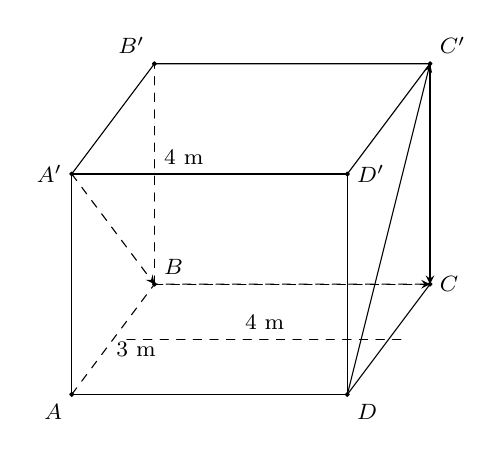
\begin{tikzpicture}[scale=0.7, font=\footnotesize, line join=round, line cap=round, >=stealth]
			\coordinate (A) at (0,0);
			\coordinate (D) at (5,0);
			\coordinate (B) at (1.5,2);
			\coordinate (C) at (6.5,2);
			\coordinate (A') at (0,4);
			\coordinate (D') at (5,4);
			\coordinate (B') at (1.5,6);
			\coordinate (C') at (6.5,6);
			
			\draw[dashed] (A) -- (B) node[midway, below right, inner sep=1pt] {$3$ m} -- (C);
			\draw[dashed] (B) -- (B') node[midway, above right] {$4$ m};
			
			\draw (A) -- (D) -- (D') -- (A') -- cycle;
			\draw (A') -- (B') -- (C') -- (D');
			\draw (D) -- (C) -- (C');
			
			\draw[dashed, ->] (A') -- (B);
			\draw[dashed, ->] (B) -- (C);
			\draw[->] (D) -- (C');
			\draw[->] (C') -- (C);
			
			\draw[dashed] (1, 1) -- (6, 1);
			\node[above] at (3.5, 1) {$4$ m};
			
			\draw [fill=black] (A) circle (1pt) node[below left] {$A$};
			\draw [fill=black] (D) circle (1pt) node[below right] {$D$};
			\draw [fill=black] (B) circle (1pt) node[above right] {$B$};
			\draw [fill=black] (C) circle (1pt) node[right] {$C$};
			\draw [fill=black] (A') circle (1pt) node[left] {$A'$};
			\draw [fill=black] (D') circle (1pt) node[right] {$D'$};
			\draw [fill=black] (B') circle (1pt) node[above left] {$B'$};
			\draw [fill=black] (C') circle (1pt) node[above right] {$C'$};
		\end{tikzpicture}
	}
	\shortans{4{,}33}
	\loigiai{
		Căn phòng là hình hộp chữ nhật $ABCD.A'B'C'D'$. Theo giả thiết ta có $AB=CD=A'B'=C'D'=3$ m, $BC=AD=B'C'=A'D'=4$ m và chiều cao $AA'=BB'=CC'=DD'=4$ m.\\
		\textbf{Phân tích chuyển động của hai con kiến}\\
		Quỹ đạo kiến 1 là $A' \to B \to C$. Độ dài đoạn đầu tiên là $A'B = \sqrt{AA'^2 + AB^2} = \sqrt{4^2 + 3^2} = 5$ m.\\
		Quỹ đạo kiến 2 là $D \to C' \to C$. Độ dài đoạn đầu tiên là $DC' = \sqrt{DD'^2 + C'D'^2} = \sqrt{4^2 + 3^2} = 5$ m.\\
		Tổ kiến ở $C$. Khi kiến 2 còn cách tổ $1$ m, nghĩa là nó đang trên đoạn $C'C$ và cách $C$ đoạn $1$ m.\\
		Quãng đường kiến 2 đã đi là $s_2 = DC' + (C'C - 1) = 5 + (4 - 1) = 8$ m.\\
		Thời gian di chuyển của kiến 2 (cũng là của kiến 1 vì xuất phát cùng lúc) là $t = \dfrac{s_2}{v_2} = \dfrac{8}{0{,}06} = \dfrac{400}{3}$ s.\\
		Trong thời gian $t$, quãng đường kiến 1 bò được là $s_1 = v_1 \cdot t = 0{,}02 \cdot \dfrac{400}{3} = \dfrac{8}{3}$ m.\\
		Vì $s_1 = \dfrac{8}{3} < A'B = 5$ nên lúc này kiến 1 vẫn đang nằm trên đoạn $A'B$.\\
		\textbf{Gắn hệ trục tọa độ và tính toán}\\
		Chọn hệ trục tọa độ $Oxyz$ sao cho gốc $O \equiv A(0;0;0)$, các tia $AD$, $AB$, $AA'$ lần lượt trùng với các tia $Ox$, $Oy$, $Oz$. Đơn vị trên mỗi trục là m.\\
		Khi đó ta có tọa độ các đỉnh $A(0;0;0)$, $D(4;0;0)$, $B(0;3;0)$, $C(4;3;0)$, $A'(0;0;4)$, $C'(4;3;4)$.\\
		Gọi $M$ là vị trí của kiến 1. Điểm $M \in A'B$ sao cho $A'M = \dfrac{8}{3}$ m.\\
		Suy ra $\overrightarrow{A'M} = \dfrac{A'M}{A'B} \overrightarrow{A'B} = \dfrac{\dfrac{8}{3}}{5} \overrightarrow{A'B} = \dfrac{8}{15} \overrightarrow{A'B}$.\\
		Ta có $\overrightarrow{A'B} = (0; 3; -4) \Rightarrow \overrightarrow{A'M} = \left(0; \dfrac{24}{15}; -\dfrac{32}{15}\right) = \left(0; \dfrac{8}{5}; -\dfrac{32}{15}\right)$.\\
		Tọa độ điểm $M$ thỏa mãn hệ
		$$ \heva{&x_M = 0 + 0 = 0 \\ &y_M = 0 + \dfrac{8}{5} = \dfrac{8}{5} \\ &z_M = 4 - \dfrac{32}{15} = \dfrac{28}{15}} \Rightarrow M\left(0; \dfrac{8}{5}; \dfrac{28}{15}\right). $$
		Gọi $N$ là vị trí của kiến 2. Điểm $N \in C'C$ và cách $C(4;3;0)$ một khoảng $1$ m.\\
		Do đường thẳng $C'C$ song song với trục $Oz$ và cao độ $z$ giảm dần từ $4$ xuống $0$, nên tọa độ $N(4; 3; 1)$.\\
		Khoảng cách giữa hai con kiến lúc này là $MN$ với
		\allowdisplaybreaks
		\begin{eqnarray*}
			MN &=& \sqrt{(4-0)^2 + \left(3 - \dfrac{8}{5}\right)^2 + \left(1 - \dfrac{28}{15}\right)^2} \\
			&=& \sqrt{16 + \left(\dfrac{7}{5}\right)^2 + \left(-\dfrac{13}{15}\right)^2} \\
			&=& \sqrt{16 + \dfrac{49}{25} + \dfrac{169}{225}} \\
			&=& \sqrt{\dfrac{3600 + 441 + 169}{225}} = \sqrt{\dfrac{4\,210}{225}} = \dfrac{\sqrt{4\,210}}{15} \approx 4{,}33\text{ m}.
		\end{eqnarray*}
	}
\end{ex}
\Closesolutionfile{ans}
